\chapter{Adding Entries}
So, there are a number of ways to enter information into the database, below we will discuss each one in turn.

\section{Albums}
\label{sect:albums}
We add data by adding albums.  Select the 
\textit{\textbf{Add Album}}
button as shown in Figure 
\ref{fig:Add album}.
\begin{figure}[!ht]
 \centering
 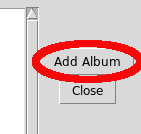
\includegraphics[scale=1]{albumButton2.png} 
 \caption{Add album}
 \label{fig:Add album}
\end{figure}

You should see the 
\textit{\textbf{New Album}}
screen (Figure 
\ref{fig:New album}).
\begin{figure}[!ht]
 \centering
 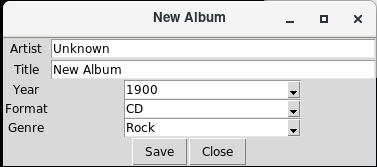
\includegraphics[scale=1]{addAlbum.png}
 \caption{New album}
 \label{fig:New album}
\end{figure} 
This is the key to entering all the data into the database.
\newpage

\subsection{The first entry}
So, let's get on and enter that first album into our new database.  You will have noticed, from Figure
\ref{fig:New album},
that some details have been pre-populated.  When a new database is created the 
\textit{\textbf{Format}}
table is populated with an entry 
\textit{\textbf{CD}}, 
and the
\textit{\textbf{Genre}} 
table is populated with an entry 
\textit{\textbf{Rock}} 
\footnote{See Part II, Tables for  full details of the Database structure.},
as a convenience to get things started.  The 
\textit{\textbf{Year}} 
drop down is populated with every year from 1900 to the current year (see Figure 
\ref{fig:Year selection}).
\begin{figure}[!ht]
 \centering
 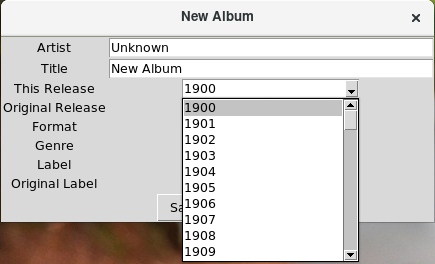
\includegraphics[scale=1]{yearDropdown.png}
 \caption{Year selection}
 \label{fig:Year selection}
\end{figure}

\newpage 
For now, just to show off a few points, select
\textbf{\textit{Save}}.
Now our main screen should look like Figure
\ref{fig:First album entered},
\begin{figure}[!ht]
 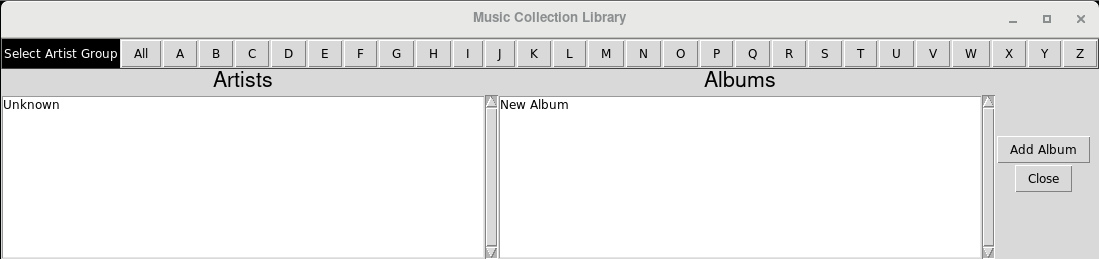
\includegraphics[width=\textwidth]{popFirstAlbum.png} 
 \caption{First album entered}
 \label{fig:First album entered}
\end{figure}
but really that's not much use to us, unless of course you have an album from 1900, on CD, in the rock genre, by a group called 'Unknown', entitled 'New Album'.  So let's change those details to something sensible. Click on the album name and you should see the
\textit{\textbf{New Album}}
screen (Figure 
\ref{fig:New album})
again.  Complete the details as shown in Figure
\ref{fig:Sgt. Pepper's Lonely Hearts Club Band}
\begin{figure}[!ht]
 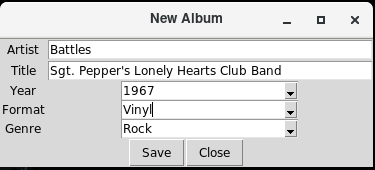
\includegraphics[scale=1]{battlespepper.png}
 \caption{Sgt. Pepper's Lonely Hearts Club Band}
 \label{fig:Sgt. Pepper's Lonely Hearts Club Band}
\end{figure}
and click 
\textbf{\textit{Save}}.
You can enter
\textbf{\textit{Vinyl}}
by just clicking in the
\textbf{\textit{Format}}
text box and overwriting the
\textbf{\textit{CD}}
text, this will add
\textbf{\textit{Vinyl}}
to the drop down 
\textbf{\textit{Format}}
menu for future use.

Looking at the main screen it seems we messed up the Artist name (unless the Beatles changed their name in some strange time jump!), this is easily fixed: double click on the artist name and you will see the screen in Figure
\ref{fig:Edit artist}.
\begin{figure}[!ht]
 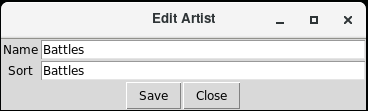
\includegraphics[scale=1]{editartist.png}
 \caption{Edit artist}
 \label{fig:Edit artist}
\end{figure} 
\newpage
Change the entries to 'Beatles', or 'The Beatles' if you prefer, see Figure
\ref{fig:Corrected artist}
\begin{figure}[!ht]
 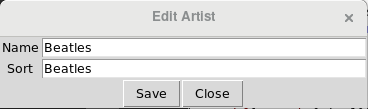
\includegraphics[scale=1]{editArtist2.png}
 \caption{Amend artist details}
 \label{fig:Corrected artist}
\end{figure} 
and click 
\textbf{\textit{Save}}.
\\You should now see something that looks like Figure
\ref{fig:Updated start screen}.
\begin{figure}[!ht]
 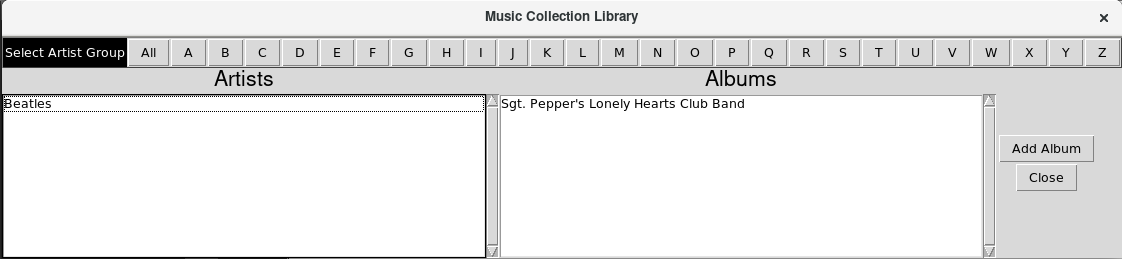
\includegraphics[width=\textwidth]{updatedMainScreen.png}
 \caption{The updated start screen}
 \label{fig:Updated start screen}
\end{figure} 
\newpage
\section{Artists}
\section{CSV}
\label{sect:csv}